\documentclass[conference]{IEEEtran}
\IEEEoverridecommandlockouts

\usepackage{cite}
\usepackage{amsmath,amssymb,amsfonts}
\usepackage{graphicx}
\usepackage{xspace}
\usepackage{complexity}
\usepackage{color}
\usepackage{comment}
\usepackage{multirow}

\graphicspath{{figs/}}
\newcommand{\todo}[1]{\textcolor{red}{[TODO: #1]}}
\newenvironment{listing}[1]{%
        \begin{list}{*}{%
%                \let\makelabel\namelistlabel
                 \settowidth{\labelwidth}{#1}%
                 \setlength{\leftmargin}{\labelwidth}%
                 \advance \leftmargin by 12pt
%                  \setlength{\labelsep}{5pt}%
                   \setlength{\itemsep}{0pt}%
%                   \setlength{\parsep}{0pt}%
%                   \setlength{\topsep}{0pt}%
%                   \setlength{\parskip}{0pt}%
}%
}{%
\end{list}}


\newcommand{\ini}{\mathrm{s}}
\newcommand{\tar}{\mathrm{t}}

\newcommand{\X}{\mathcal{X}}
\newcommand{\Z}{\mathcal{Z}}
\newcommand{\sets}{\mathcal{S}}
\newcommand{\zind}{\mathcal{Z}_{\mathrm{ind}}}
\newcommand{\zsol}{\mathcal{Z}_{\mathrm{sol}}}
\newcommand{\labeln}{\mathsf{label}}
\newcommand{\rootn}{\mathsf{root}}
\newcommand{\child}[1]{\mathsf{child}_{#1}}
\newcommand{\remove}{\mathsf{remove}}
\newcommand{\add}{\mathsf{add}}
\newcommand{\swap}{\mathsf{swap}}

\newcommand{\OrigDecom}{\textsf{orig}\xspace}
\newcommand{\HeurDecom}{\textsf{heur}\xspace}
\newcommand{\OptDecom}{\textsf{opt}\xspace}

\newcommand{\TJ}{\textsc{Token Jumping}\xspace}
\newcommand{\satisfiability}{\textsc{SAT}\xspace}
\newcommand{\SR}{\textsc{SAT Reconfiguration}\xspace}
\newcommand{\LCR}{\textsc{List Coloring Reconfiguration}\xspace}
\newcommand{\SPR}{\textsc{Shortest Path Reconfiguration}\xspace}

\newcommand{\SATseries}{\textsc{SAT} series\xspace}
\newcommand{\LCseries}{\textsc{LC} series\xspace}
\newcommand{\SPseries}{\textsc{SP} series\xspace}
\newcommand{\ISseries}{\textsc{IS} series\xspace}

\newcommand{\XSAT}{\textsc{SAT}\xspace}
\newcommand{\XLC}{\textsc{LC}\xspace}
\newcommand{\XSP}{\textsc{SP}\xspace}
\newcommand{\XIS}{\textsc{IS}\xspace}
\newcommand{\XRAND}{\textsc{RAND}\xspace}

\newcommand{\snumfun}[1]{s_{#1}}
\newcommand{\snum}[2]{\snumfun{#1}(#2)}

\newcommand{\KJ}[2]{{\color{red} #2}}
\newcommand{\KJQ}[1]{{\color{blue} #1}}

\begin{document}

\title{Efficiency of ZDD-Based Analyses for Independent Set Reconfiguration: A Pathwidth-Centric Study\thanks{This work was supported by JSPS KAKENHI Grant Numbers JP24H00686, JP24H00690, and JP23K12974.}}

\author{
\IEEEauthorblockN{Kanae Sawamura}
\IEEEauthorblockA{\textit{Graduate School of Information Sciences}\\
\textit{Tohoku University}\\
Sendai, Japan\\
sawamura.kanae.r7@dc.tohoku.ac.jp}
\and
\IEEEauthorblockN{Takehide Soh}
\IEEEauthorblockA{\textit{Graduate School of Informatics}\\
\textit{Nagoya University}\\
Nagoya, Japan\\
soh@i.nagoya-u.ac.jp}
\and
\IEEEauthorblockN{Yasuaki Kobayashi}
\IEEEauthorblockA{\textit{Faculty of Information Science and Technology}\\
\textit{Hokkaido University}\\
Sapporo, Japan\\
koba@ist.hokudai.ac.jp}
\and
\IEEEauthorblockN{Yuma Tamura}
\IEEEauthorblockA{\textit{Graduate School of Information Sciences}\\
\textit{Tohoku University}\\
Sendai, Japan}
\and
\IEEEauthorblockN{Yuta Nozaki}
\IEEEauthorblockA{\textit{Faculty of Environment and Information Sciences}\\
\textit{Yokohama National University}\\
Yokohama, Japan\\
\textit{WPI-SKCM$^2$, Hiroshima University}\\
Hiroshima, Japan\\
nozaki-yuta-vn@ynu.ac.jp}
\and
\IEEEauthorblockN{Jun Kawahara}
\IEEEauthorblockA{\textit{Graduate School of Informatics}\\
\textit{Kyoto University}\\
Kyoto, Japan\\
jkawahara@i.kyoto-u.ac.jp}
\and
\IEEEauthorblockN{Takehiro Ito}
\IEEEauthorblockA{\textit{Graduate School of Information Sciences}\\
\textit{Tohoku University}\\
Sendai, Japan\\
takehiro@tohoku.ac.jp}
}

\maketitle

\begin{abstract}
Zero-suppressed binary decision diagrams (ZDDs) are a standard data structure for
compactly representing families of combinatorial solutions, and controlling the
pathwidth of the input graph is known to be effective for keeping ZDDs small when
they are constructed.
In combinatorial reconfiguration, however, a ZDD-based solver must repeatedly
perform transition computations on top of a solution-space ZDD, and it has
remained unclear how much pathwidth affects the performance of such solvers.
This paper investigates the impact of path decomposition as a preprocessing step
for ZDD-based solvers for the independent set reconfiguration (ISR) problem under
the token jumping rule.
We integrate path decomposition into \textsc{ddreconf}, a state-of-the-art
ZDD-based ISR solver, by reordering the input edges according to a computed
decomposition, and we analyze how this reduces ZDD size both at construction time
and during reconfiguration.
Computational experiments on the shortest and farthest variants show that the
proposed preprocessing consistently improves the performance of
\textsc{ddreconf}.
Moreover, even heuristic path decompositions that do not necessarily minimize
pathwidth are sufficient to obtain substantial speedups in practice.
\end{abstract}

\begin{IEEEkeywords}
Combinatorial reconfiguration, independent set reconfiguration, zero-suppressed binary decision diagram, path decomposition, pathwidth
\end{IEEEkeywords}

\section{Introduction}
Combinatorial reconfiguration studies how one feasible solution of a
combinatorial problem can be transformed into another through a sequence of small
local changes~\cite{nishimura18}.
Among these problems, independent set reconfiguration (ISR) asks whether one
independent set of a graph can be transformed into another by a sequence of small
changes that keeps an independent set at every step.
In this paper we adopt the token jumping rule, in which each step moves a single
token to another vertex, equivalently, removes one vertex from the current
independent set and adds one vertex outside it; this is the rule used in the CoRe
Challenge.
ISR is PSPACE-complete in general~\cite{kamemi12,itdehapasiueun11}, and developing
practically efficient solvers remains an active research topic.

Zero-suppressed binary decision diagrams (ZDDs) provide a compact implicit
representation of a family of sets and have been successfully applied to a wide
range of combinatorial problems.
It is well known that the size of a ZDD built from a graph is closely related to
the pathwidth of the graph: a smaller pathwidth often leads to a smaller
ZDD~\cite{inoue16}.
This observation has motivated path-decomposition-based techniques in many ZDD
applications.

ZDD-based solvers for reconfiguration problems, however, follow a different
workflow.
They first construct a ZDD representing the entire solution space and then
repeatedly execute transition operations on this ZDD to search for a
reconfiguration sequence.
Although pathwidth is recognized as an important parameter for the initial ZDD
construction, its effect on the overall performance of reconfiguration solvers,
including the cost of the intermediate ZDD operations during the search, has not
been systematically studied.

In this paper, we focus on ISR under the token jumping rule and analyze how a
path decomposition of the input graph, used as preprocessing, affects ZDD-based
reconfiguration solvers.
The input to the CoRe Challenge solvers is a graph given as an ordered list of
edges, and the state-of-the-art ZDD-based solver \textsc{ddreconf} processes
these edges in the given order; this order determines the width of the path
decomposition that the solver implicitly works with, and hence the sizes of the
ZDDs it builds and manipulates.
Our preprocessing simply reorders the edges according to a path decomposition of
small width, leaving the solver itself untouched.
We study two variants that probe the solution space in complementary ways: the
shortest variant, which seeks a shortest reconfiguration sequence between two
given independent sets, and the farthest variant, which seeks an independent set
farthest from a given one.
Our main contributions are as follows:
\begin{itemize}
\item We analyze the effect of a path decomposition of the input graph, used as a
preprocessing step, on ZDD-based ISR solvers, covering both the construction of
the solution-space ZDD and the transition computation during reconfiguration.
\item Through computational experiments, we show that integrating the proposed
preprocessing into the ZDD-based solver \textsc{ddreconf} improves its
performance on both the shortest and farthest variants.
\item We demonstrate that optimal minimization of pathwidth is not necessary in
practice: heuristic path decompositions already yield sufficient performance
gains.
\end{itemize}

The remainder of this paper is organized as follows.
Section~\ref{sec:preliminaries} introduces ISR and reviews ZDD-based solvers.
Section~\ref{sec:approach} presents our path-decomposition-based approach and its
integration with \textsc{ddreconf}.
Section~\ref{sec:analysis} analyzes why ZDD-based solvers suffer from large ZDD
sizes and how path decomposition mitigates this issue.
Section~\ref{sec:experiments} reports experimental results.
Section~\ref{sec:conclusion} concludes the paper.



\section{Preliminaries}
\label{sec:preliminaries}

\subsection{Independent Set Reconfiguration}
\label{subsec:isr}

%\begin{itemize}
%\item Definition of the independent set reconfiguration (ISR) problem under Token jumping rule. Shortest/longest variants.
%\item Complexity (PSPACE-completeness) and relationship to combinatorial reconfiguration.
%\item Benchmark instances used in this paper (e.g., CoRe Challenge).
%\end{itemize}

Let $G=(V,E)$ be an undirected graph, where $V$ is the set of vertices and $E$
is the set of edges. A vertex subset $I\subseteq V$ is an \emph{independent set
of $G$} if no two vertices in $I$ are adjacent in $G$.
Henceforth, we refer to each vertex contained in an independent set as a
\emph{token}.
Two independent sets $I$ and $I'$ of $G$ are \emph{adjacent} under the
\emph{Token Jumping} (TJ) rule if $|I \bigtriangleup I'| = 2$, namely, $I'$ can
be obtained from $I$ by moving a single token in $I$ to another vertex that is
not in $I$, and vice versa.
Then, for two independent sets $I_\ini$ and $I_\tar$ of $G$ such that
$|I_\ini|=|I_\tar|$, a \emph{reconfiguration sequence} between $I_\ini$ and
$I_\tar$ is a sequence $\langle I_0, I_1, \ldots, I_\ell \rangle$ such that:
\begin{listing}{-}
\item[-] $I_0 = I_\ini$ and $I_\ell = I_\tar$;
\item[-] $I_i$ is an independent set of $G$ such that $|I_i| = |I_\ini| = |I_\tar|$, for each $i$, $0 \leq i \leq \ell$;
\item[-] $I_i$ and $I_{i+1}$ are adjacent under TJ for each $i$, $0 \le i \le \ell-1$.
\end{listing}
Then, the \emph{Independent Set Reconfiguration Problem} (ISRP) under TJ is to
determine whether there exists a reconfiguration sequence between $I_\ini$ and
$I_\tar$. This problem is known to be \PSPACE-complete~\cite{kamemi12}.
The \PSPACE-completeness implies that there are yes-instances such that even a
shortest reconfiguration sequence has super-polynomial length, under the
assumption that $\PSPACE \neq \NP$.

In this paper, we study two variants of ISRP under TJ, which probe the structure
of the solution space in complementary ways.
The \emph{solution space} of an ISR instance $(G, I_\ini, I_\tar)$ is the graph whose nodes are the
independent sets of $G$ of size $|I_\ini|$ and in which two independent sets are
joined whenever they are adjacent under TJ; a reconfiguration sequence is exactly
a path in this graph. The \emph{distance} between two independent sets in the
solution space is the length of a shortest reconfiguration sequence between them;
or it is $\infty$ if no such sequence exists. The solution space can be exponentially
large in $|V|$, which makes designing practically efficient solvers a challenging
task.

The first is the \emph{shortest variant}, which generalizes ISRP.
Given an ISRP instance $(G, I_\ini, I_\tar)$, the shortest variant aims to
determine the existence of a reconfiguration sequence between $I_\ini$ and
$I_\tar$ and, if so, to compute the distance between them. This is the classical
reachability/shortest-path question between two prescribed independent sets in the solution space,
which has been studied extensively from a theoretical standpoint and was adopted
as a metric of the CoRe Challenge~\cite{sotaokit24}.

The second is the \emph{farthest variant}~\cite{ItoKNSSTT23}.
Given only one independent set $I_\ini$, the farthest variant aims to find an
independent set whose distance from $I_\ini$ is maximum among all independent
sets reachable from $I_\ini$, together with that distance. Rather than connecting
two prescribed independent sets, this variant asks how far the reconfiguration
relation can carry $I_\ini$ throughout its connected component of the solution
space. It is therefore a one-to-many question about the extent of a connected
component, in contrast to the one-to-one, path-between-two-endpoints nature of
the shortest variant. Studying both lets us observe how pathwidth affects a
ZDD-based solver on two qualitatively different uses of the same solution-space
representation.

\subsection{Overview of ZDD-Based Solvers}
\label{subsec:zdd_solver}

%\begin{itemize}
%\item Brief review of ZDDs and their use in representing families of independent sets.
%\item Overview of \textsc{ddreconf} and the general workflow: solution-space ZDD construction followed by repeated transition computation.
%\item Role of variable ordering and graph structure in ZDD size.
%\end{itemize}

A \emph{zero-suppressed binary decision diagram} (ZDD) is a directed acyclic
graph that compactly represents a family of sets over a fixed universal set
$U = \{x_1, \dots, x_n\}$ equipped with a total order $x_1 < \cdots < x_n$.
It has two terminal nodes $\bot$ and $\top$, representing the empty family
$\emptyset$ and the family $\{\emptyset\}$, respectively, and each non-terminal
node is labeled with an element of $U$ and has a $0$-arc and a $1$-arc.
By sharing isomorphic subgraphs and suppressing redundant nodes, a ZDD can
represent a family whose cardinality is exponential in $n$ using far fewer
nodes, and it supports efficient family operations such as union,
intersection, and difference through recursive procedures over its shared
structure~\cite{Minato1993,knuth:taocp41}.

For ISRP, the relevant family is the set of all independent sets of the input
graph $G = (V, E)$, where the universal set is taken to be the vertex set $V$.
The state-of-the-art ZDD-based solver \textsc{ddreconf}~\cite{ItoKNSSTT23} solves
ISRP under the TJ rule in two phases.

In the first phase, the solver constructs the \emph{solution-space ZDD}.
It first builds a ZDD $\zind$ representing the family of all independent sets of
$G$~\cite{Hayase1995}. Recall that, under the TJ rule, every independent set in a
reconfiguration sequence has the same cardinality $k = |I_\ini|$ as the start
independent set $I_\ini$. The solver therefore builds a ZDD $\Z_{=k}$
representing all vertex subsets of cardinality exactly $k$~\cite{knuth:taocp41},
and obtains the solution space as $\zsol = \zind \cap \Z_{=k}$, which represents
every independent set of $G$ of cardinality $k$. The family $\sets(\zsol)$ is
exactly the node set of the solution space defined in
Section~\ref{subsec:isr}.

In the second phase, the solver repeatedly performs \emph{transition
computation} on top of $\zsol$. Starting from $\Z^{0}$ with
$\sets(\Z^{0}) = \{I_\ini\}$, it iteratively computes
\begin{equation}
  \Z^{i} \;\gets\; \mathsf{op}(\Z^{i-1}) \cap \zsol,
  \label{eq:transition}
\end{equation}
where $\mathsf{op}$ applies the TJ rule to every independent set encoded by
$\Z^{i-1}$. Concretely, $\mathsf{op}(\Z) = \swap(\Z, V, V)$, where
$\swap(\Z, A, R)$ represents the family
\[
  \{\, I \cup \{v\} \setminus \{v'\} \mid I \in \sets(\Z),\,
  v \in A \setminus I,\, v' \in I \cap R \,\}
\]
obtained by moving a single token, and intersecting with $\zsol$ retains only
those sets that are independent sets of cardinality $k$. Hence $\Z^{i}$
represents exactly the family of independent sets whose distance from $I_\ini$ is
$i$, and iterating \eqref{eq:transition} amounts to a breadth-first search over
the solution space. This implicit search lets \textsc{ddreconf} explore an
exponentially large solution space, since each $\Z^{i}$ may encode an enormous
number of independent sets within a small ZDD.

Both variants are answered from this sequence of ZDDs. For the shortest variant,
the solver checks $\Z^{i}$ after each step: once $I_\tar \in \sets(\Z^{i})$, the
distance between $I_\ini$ and $I_\tar$ is $i$, and once $\Z^{i} = \bot$ without
having reached $I_\tar$, no reconfiguration sequence exists. For the farthest
variant, the solver continues until $\Z^{h+1} = \bot$; the last nonempty
$\Z^{h}$ then contains the independent sets farthest from $I_\ini$, and $h$ is
their distance.

The performance of this workflow is governed by the \emph{size} (number of
nodes) of the ZDDs that appear in it, which in turn depends critically on the
order in which the edges of $G$ are processed during ZDD construction. For the
first phase, this dependence is well understood~\cite{inoue16}: the working state
maintained during top-down ZDD construction, and hence both the construction
time and the resulting ZDD size, grows rapidly with the width of the path
decomposition induced by the processing order (we make this correspondence
precise in Section~\ref{subsec:pathdecomp}). A processing order of small width
therefore keeps $\zind$, and hence $\zsol$, compact; for example, the family of
independent sets of an $8 \times 250$ grid graph has cardinality
$3.07 \times 10^{361}$, yet it can be represented by a ZDD with only $49{,}989$
nodes under a suitable order~\cite{ItoKNSSTT23}. Crucially, \textsc{ddreconf}
fixes a single processing order before construction and reuses it throughout
both phases. While the effect of this order on the first phase is thus inherited
from established results on ZDD construction, its effect on the \emph{second}
phase has not been systematically studied. This second-phase effect concerns the
sizes of the intermediate ZDDs $\Z^{i}$ generated during reconfiguration, and
consequently the overall running time of the solver. This gap motivates our study
of how the processing order, which we derive from a path decomposition of $G$,
affects the end-to-end performance of ZDD-based reconfiguration.



\section{Our Approach}
\label{sec:approach}

%\subsection{Path Decomposition and the Input Edge Order}
%\begin{itemize}
%\item Definition of path decomposition and pathwidth.
%\item Overview of the path-decomposition-based preprocessing algorithm.
%\item How the decomposed structure is used to determine a variable ordering for ZDD construction.
%\item Exact vs.\ heuristic path decomposition methods used in this paper.
%\end{itemize}

%\subsection{Integration with \textsc{ddreconf}}
%\begin{itemize}
%\item How path decomposition is incorporated into the \textsc{ddreconf} framework as a preprocessing step.
%\item Implementation details relevant to reconfiguration (variable ordering, interface between preprocessing and the solver).
%\item Summary of the overall algorithm pipeline.
%\end{itemize}


Our approach is built on a simple observation made in
Section~\ref{subsec:zdd_solver}: the performance of \textsc{ddreconf} is governed
by the sizes of the ZDDs that appear throughout its two phases, and these sizes
are determined by the order in which the edges of the input graph $G$ are
processed during ZDD construction. We already know that, for the first phase, a
processing order of small width keeps the constructed ZDD small; what is not
understood is how the order affects the \emph{second} phase, that is, the sizes
of the intermediate ZDDs $\Z^{i}$ generated during reconfiguration, and hence the
end-to-end performance of the solver. The original \textsc{ddreconf} fixes the
order according to the input itself and never revisits it. We instead treat the
order as a tunable \emph{preprocessing} parameter derived from a path
decomposition of $G$, and feed the resulting order to \textsc{ddreconf} without
modifying the solver. Concretely, we compare three orders of increasing quality
and preprocessing cost: \OrigDecom, the order already present in the input;
\HeurDecom, an order obtained from a heuristic path decomposition; and
\OptDecom, an order obtained from a minimum-width path decomposition. This
section formalizes the path-decomposition view of the input order
(Section~\ref{subsec:pathdecomp}), describes the heuristic and exact algorithms
behind \HeurDecom and \OptDecom (Section~\ref{subsec:algorithms}), and explains
how the preprocessing is integrated into the \textsc{ddreconf} pipeline
(Section~\ref{subsec:integration}).

\subsection{Path Decomposition and the Input Edge Order}
\label{subsec:pathdecomp}

We first recall the standard definitions.
A \emph{path decomposition} of a graph $G = (V, E)$ is a sequence
$(X_1, \dots, X_\ell)$ of subsets of $V$, called \emph{bags}, such that
(i) for every edge $\{u, v\} \in E$ there is a bag $X_i$ with $u, v \in X_i$, and
(ii) for every vertex $v \in V$, the bags containing $v$ form a contiguous
subsequence. The \emph{width} of a path decomposition is
$\max_{1 \le i \le \ell} |X_i| - 1$, and the \emph{pathwidth} $\mathrm{pw}(G)$ of
$G$ is the minimum width over all its path decompositions.

The CoRe Challenge provides each instance as an input graph in the DIMACS
format~\cite{sotaokit24}: a \texttt{p} line declares the numbers of vertices and
edges, and each subsequent \texttt{e} line lists the two endpoints of an edge.
When \textsc{ddreconf} reads such a file and constructs $\zind$ in the first
phase, it processes the edges one by one, in the order in which they appear in
the file. The cost of this top-down construction is governed by the
\emph{frontier}, the set of vertices that are incident to both already-processed
and not-yet-processed edges; it is a folklore fact, made explicit by Inoue and
Minato~\cite{inoue16}, that the maximum frontier size over the construction
coincides with the width of a path decomposition of $G$ determined by the edge
order. Moreover, given an edge order, the width of this associated path
decomposition can be computed by the algorithm of Kobayashi and
Nakahata~\cite[Lemma~2]{KobayashiNakahata2020}. Through this correspondence we
treat an edge order and the width of its path decomposition interchangeably, so
that quantities stated in terms of pathwidth apply equally to the edge orders
that \textsc{ddreconf} actually consumes.

Consequently, the order in which edges are listed in the input file, an artifact
of how each instance happens to be encoded, directly determines the width of the
path decomposition that \textsc{ddreconf} implicitly works with, and hence the
sizes of the ZDDs it builds and manipulates. For the first phase, the effect is
well understood: a smaller width keeps $\zind$, and hence $\zsol$, compact
(Section~\ref{subsec:zdd_solver}). The open question, and the subject of this
paper, is how the same edge order propagates to the second phase, that is, to the
sizes of the intermediate ZDDs $\Z^{i}$ and the overall running time. This leads
to a natural plan: \emph{replace the input edge order with one derived from a
path decomposition of small width, and measure how the performance of
\textsc{ddreconf} changes across both phases.}

\subsection{Heuristic and Optimal Path Decomposition}
\label{subsec:algorithms}

Computing $\mathrm{pw}(G)$ exactly is NP-hard, so obtaining a minimum-width path
decomposition is expensive in general. Besides the decomposition induced by the
input order (\OrigDecom), we obtain a path decomposition using the algorithm of
Kobayashi, Komuro, and Tamaki~\cite{KobayashiKomuroTamaki2014}. This algorithm
computes an optimal path decomposition by reducing the search space through
commitments and gradually narrowing down to minimum width; it produces a first
feasible decomposition quickly and, if run to completion, eventually returns an
optimal one. We exploit both ends of this process, yielding two path
decompositions of different quality and cost. This algorithm is an existing
method, which we use as is and do not claim as a contribution of this paper.

\paragraph{Heuristic decomposition (\HeurDecom).}
As a fast preprocessing step, we take the first decomposition that the algorithm
produces, whose width is small but not necessarily minimum. Obtaining it is
quick enough to serve as a lightweight preprocessor even on the larger CoRe
Challenge instances. Because this first decomposition is not guaranteed to attain
the minimum width, it is occasionally wider than the one induced by the original
input order. Since the width of the original order is itself available
(Section~\ref{subsec:pathdecomp}), we compare the two and keep the better one:
only when the first decomposition is strictly wider than the original do we fall
back to the original order. Thus \HeurDecom never yields a wider decomposition
than \OrigDecom.

\paragraph{Optimal decomposition (\OptDecom).}
To examine the effect of attaining the true minimum width, we run the same
algorithm to completion, obtaining an optimal path decomposition, i.e., one of
width exactly $\mathrm{pw}(G)$. This is far more time-consuming than obtaining the
first decomposition, and is prohibitively so for some instances, but it lets us
measure the best possible gain achievable through path-decomposition-based
reordering and compare it against \HeurDecom.

\subsection{Integration with \textsc{ddreconf} and the Three Decompositions}
\label{subsec:integration}

In all three cases, the path decomposition is used purely as preprocessing: from
the decomposition we derive an edge order, write it back as a reordered DIMACS
file, and run the unmodified \textsc{ddreconf} on it. The solver itself is
identical across all runs, including its solution-space ZDD construction, its
swap-based transition computation, and its breadth-first reconfiguration search;
only the order in which the edges of $G$ are presented differs. This makes the
comparison clean: any difference in running time, memory usage, or
solved-instance count is attributable solely to the edge order, and hence to the
underlying path decomposition.

We compare the following three path decompositions.
\begin{description}
  \item[\OrigDecom:] the path decomposition induced by the edge order as given in
    the CoRe Challenge input file, used without any reordering. This is the
    baseline and corresponds to the original \textsc{ddreconf} behavior.
  \item[\HeurDecom:] a path decomposition of small but not necessarily minimum
    width, computed by the heuristic algorithm~\cite{KobayashiKomuroTamaki2014};
    if it is strictly wider than \OrigDecom, we fall back to the original order,
    so that \HeurDecom is never wider than \OrigDecom.
  \item[\OptDecom:] an optimal (minimum-width) path decomposition, computed by an
    exact algorithm.
\end{description}
For \HeurDecom and \OptDecom, we derive an edge order from the computed path
decomposition and run \textsc{ddreconf} on that order. The preprocessing cost
increases sharply along this list: \OrigDecom incurs none, \HeurDecom adds only
a fast preprocessing step, whereas \OptDecom can be extremely time-consuming.
Section~\ref{sec:experiments} reports how these three path decompositions compare
in practice, and in particular whether the inexpensive \HeurDecom decomposition
already captures most of the benefit that the costly \OptDecom decomposition
provides.


\section{Experimental Results}
\label{sec:experiments}

\subsection{Experimental Setup}
\label{subsec:setup}

We implemented the path-decomposition preprocessing on top of
\textsc{ddreconf}~\cite{ItoKNSSTT23} and evaluated the three orders
\OrigDecom, \HeurDecom, and \OptDecom defined in Section~\ref{sec:approach}.
%% TODO: machine spec (CPU, RAM), compiler, ZDD libraries and versions,
%% ddreconf version/commit, and the implementation used for the pathwidth
%% computation of Kobayashi--Komuro--Tamaki.
All experiments were run on \todo{machine and software environment}.

\paragraph{Benchmarks.}
We used the benchmark instances of the CoRe Challenge 2022 and
2023~\cite{sotaokit24}. In total there are $616$ instances arising from $455$
distinct input graphs; each graph may appear in several instances that differ in
the start and goal independent sets.
%% TODO: how instances were selected (all? a subset?), and the range of
%% graph sizes; any series included/excluded.
The graphs range widely in size, from tens of vertices to graphs with more than
$10^{6}$ edges \todo{confirm size range and selection criteria}.

\paragraph{Time limits.}
We adopt a two-stage time budget that separates preprocessing from solving.
Computing \OptDecom requires solving an NP-hard pathwidth problem, so we allow up
to one hour for this computation; if it does not finish within the limit, no
optimal order is available for that instance and \OptDecom is undefined.
Computing \HeurDecom and reading the input order for \OrigDecom incur negligible
preprocessing cost.
Given the (possibly reordered) input, we then run the unmodified
\textsc{ddreconf} with a time limit of $30$ minutes of wall-clock time per
instance. An instance is counted as \emph{solved} under a given order if
\textsc{ddreconf} terminates with the correct answer within this $30$-minute
limit.
We report results for both the shortest and the farthest variant.

Of the $455$ graphs, the optimal pathwidth (and hence \OptDecom) was computed
within the one-hour limit for $262$ graphs, corresponding to $329$ of the $616$
instances; for the remaining $193$ graphs ($287$ instances) the optimal order
could not be obtained.
This split is itself informative: the instances for which \OptDecom is available
are markedly smaller (median $138$ vertices and $638$ edges) than those for which
it is not (median $450$ vertices and $3218$ edges). We therefore present two
kinds of comparison: one restricted to the instances on which all three orders
are available, and one over all instances that contrasts \OrigDecom with
\HeurDecom.

\subsection{Pathwidth of the Three Orders}
\label{subsec:pw-three}

Before turning to solver performance, we examine how much the three orders differ
in width on the input graphs themselves, independently of whether the instances
are solved.
Figure~\ref{fig:pw-three} shows, for each of the $262$ graphs whose optimal
pathwidth was computed within the one-hour limit, the pathwidth of \OrigDecom,
\HeurDecom, and \OptDecom, with the three values for the same graph connected by
a vertical line.
Two observations stand out.
First, reordering the edges by a path decomposition reduces the width
dramatically: the median pathwidth drops from $46$ for \OrigDecom to $11$ for
both \HeurDecom and \OptDecom.
Second, \HeurDecom is already very close to \OptDecom; the two markers nearly
coincide for most graphs, and the median ratio of their widths is $1.00$.
In other words, on this benchmark the heuristic decomposition attains
essentially the same width as the optimal one, while costing far less to compute
(Section~\ref{subsec:solved}).
Many graphs that have width on the order of $100$ under the input order collapse
to a narrow band of width around $10$ to $17$ once decomposed, even when the
graph is large.

\begin{figure}[t]
  \centering
  %% TODO: final vector figure; recolor to avoid clashing with the
  %% solved/unsolved colors used in Fig.~\ref{fig:pw-solvability}.
  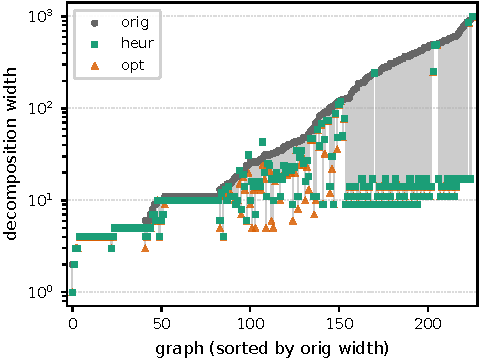
\includegraphics[width=\linewidth]{pw_three_orders.pdf}
  \caption{Pathwidth of \OrigDecom, \HeurDecom, and \OptDecom for each input
  graph (the $262$ graphs whose optimal pathwidth was computed within one hour).
  The three values for the same graph are joined by a vertical line.
  \HeurDecom (square) and \OptDecom (triangle) almost coincide, well below
  \OrigDecom (circle).}
  \label{fig:pw-three}
\end{figure}

\subsection{Effect on the Solution-Space ZDD}
\label{subsec:zddsize}

We next measure how the reduced width translates into a smaller solution-space
ZDD, i.e., the ZDD $\zsol$ built in the first phase of \textsc{ddreconf}.
To compare the three orders on a common footing, we restrict attention to the
instances solved by all three orders within the time limit ($208$ instances for
the shortest variant and $206$ for the farthest variant), so that every order
produces a value for every instance.
%% TODO: revisit whether to restrict to commonly solved instances; also report
%% the maximum, not only central tendency, since solving large-width instances
%% is itself a key benefit.
Table~\ref{tab:zddsize} reports, for each order and each variant, the median
pathwidth, the geometric mean of the solution-space ZDD size, the geometric mean
of the first-phase construction time, and the geometric mean of the peak memory.

\begin{table}[t]
  \centering
  \caption{Solution-space ZDD and first-phase cost on the instances solved by all
  three orders ($208$ for shortest, $206$ for farthest). Values are geometric
  means except for pathwidth (median).}
  \label{tab:zddsize}
  \begin{tabular}{llrrrr}
    \hline
    variant & order & pathwidth & ZDD size & constr.\ time [s] & memory [kB] \\
    \hline
    \multirow{3}{*}{shortest}
      & \OrigDecom & $31$ & $2867$ & $0.178$ & $288{,}755$ \\
      & \HeurDecom & $11$ & $1138$ & $0.079$ & $179{,}456$ \\
      & \OptDecom  & $10$ & $\phantom{0}920$ & $0.070$ & $160{,}581$ \\
    \hline
    \multirow{3}{*}{farthest}
      & \OrigDecom & $31$ & $2668$ & $0.155$ & $307{,}523$ \\
      & \HeurDecom & $11$ & $1105$ & $0.076$ & $193{,}464$ \\
      & \OptDecom  & $10$ & $\phantom{0}898$ & $0.067$ & $168{,}404$ \\
    \hline
  \end{tabular}
\end{table}

The solution-space ZDD shrinks monotonically as the width decreases, for both
variants.
For the shortest variant, relative to \OrigDecom the per-instance reduction in
ZDD size has a geometric mean of $2.52\times$ for \HeurDecom and $3.12\times$ for
\OptDecom; the corresponding reductions in first-phase construction time and peak
memory are $2.0\times$ and $1.6\times$ for \HeurDecom, and $2.4\times$ and
$1.8\times$ for \OptDecom. The farthest variant shows the same pattern
($2.42\times$ and $2.97\times$ in ZDD size for \HeurDecom and \OptDecom).
Across these commonly solved instances, smaller width is consistently associated
with a smaller solution-space ZDD: the Spearman rank correlation between
pathwidth and ZDD size is $0.65$, and that between ZDD size and total solving
time is $0.52$.
As in the pathwidth comparison, \HeurDecom captures most of the benefit of
\OptDecom: it reaches roughly $80\%$ of the optimal width reduction and a
comparable shrinkage of the solution-space ZDD.

\subsection{Solved Instances and Running Time}
\label{subsec:solved}

We now turn to the bottom-line question of how many instances each order lets
\textsc{ddreconf} solve within the $30$-minute limit.
Table~\ref{tab:solved} reports the counts for both variants, under the two
comparisons motivated in Section~\ref{subsec:setup}.

\begin{table}[t]
  \centering
  \caption{Number of instances solved within $30$ minutes. The left block is
  restricted to the $329$ instances for which all three orders are available; the
  right block is over all $616$ instances, where \OptDecom is available for only
  $329$ of them.}
  \label{tab:solved}
  \begin{tabular}{lrrr|rr}
    \hline
    & \multicolumn{3}{c|}{opt-available ($329$)} & \multicolumn{2}{c}{all ($616$)} \\
    variant & \OrigDecom & \HeurDecom & \OptDecom & \OrigDecom & \HeurDecom \\
    \hline
    shortest & $210$ & $219$ & $218$ & $210$ & $229$ \\
    farthest & $208$ & $218$ & $218$ & $208$ & $227$ \\
    \hline
  \end{tabular}
\end{table}

On the instances where all three orders are available, both \HeurDecom and
\OptDecom solve more than \OrigDecom, and \HeurDecom is on par with \OptDecom
(for the shortest variant, $219$ versus $218$; for the farthest variant, $218$
versus $218$).
Over all instances, \HeurDecom solves the most: $229$ versus $210$ for
\OrigDecom on the shortest variant, and $227$ versus $208$ on the farthest
variant.

The reason \HeurDecom outperforms \OptDecom overall lies in preprocessing cost.
On the instances where \OptDecom is available, computing \HeurDecom takes a
median of $2.1$ seconds (at most $13.7$ seconds), whereas computing \OptDecom
takes a median of $3.2$ seconds but a mean of $64.7$ seconds and up to
$2348$ seconds.
More importantly, for $287$ of the $616$ instances the optimal pathwidth could
not be computed within one hour at all, so \OptDecom never reaches the solver on
these instances.
These are exactly the large, hard instances: under \OrigDecom, \textsc{ddreconf}
solves \emph{none} of these $287$ instances within $30$ minutes, whereas under
\HeurDecom it solves $10$ of them (shortest) and $9$ of them (farthest).
Thus the lightweight heuristic decomposition is not merely a cheaper substitute
for the optimal one; it is the only one of the three that reaches these instances
at all.

Because the solution-space ZDD construction is shared by both variants, the two
variants differ only in the second phase, where the farthest variant explores the
solution space until it is exhausted.
This makes the farthest variant somewhat more expensive in the second phase, and
correspondingly a few fewer instances are solved under it; otherwise the two
variants exhibit the same trends.

\subsection{Pathwidth Determines Solvability}
\label{subsec:solvability}

Finally, we examine which property of an instance governs whether it can be
solved.
Figure~\ref{fig:pw-solvability} plots every instance by its number of edges and
the pathwidth of the order used, marking whether \textsc{ddreconf} solves it
within $30$ minutes, for \OrigDecom (left) and \HeurDecom (right).
In both panels, solved and unsolved instances separate along an almost horizontal
boundary: solvability is governed by pathwidth rather than by graph size.
Large graphs are solved when their pathwidth is small and left unsolved when it
is large; among graphs with more than the median number of edges, those solved
under \HeurDecom have a median pathwidth of $17$, while those left unsolved have a
median pathwidth of $154$.
Comparing the two panels shows the effect of preprocessing: \HeurDecom pulls the
same graphs downward into the low-pathwidth, solvable region, turning many
instances that are unsolved under \OrigDecom into solved ones.
Quantitatively, the (point-biserial) correlation between solvability and
pathwidth is stronger than that between solvability and the number of edges
($-0.63$ versus $-0.55$ for \HeurDecom), confirming that pathwidth is the better
predictor.

\begin{figure}[t]
  \centering
  %% TODO: final vector figure; the farthest variant shows the same trend and is
  %% omitted to save space (state this if a reviewer asks).
  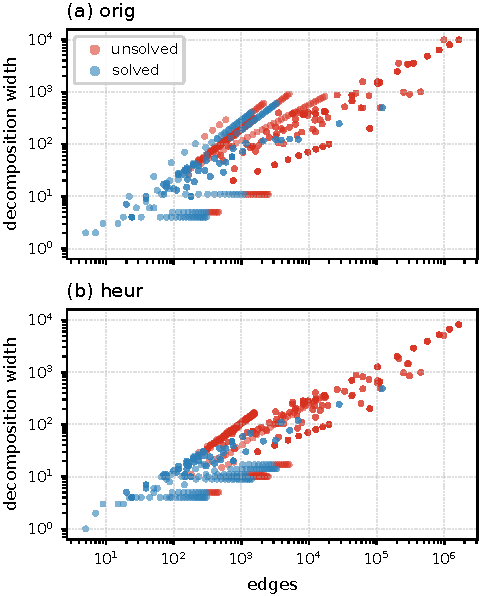
\includegraphics[width=\linewidth]{pw_solvability.pdf}
  \caption{Each instance plotted by number of edges and the pathwidth of its
  order, for \OrigDecom (left) and \HeurDecom (right), on the shortest variant.
  Solved instances (within $30$ minutes) lie below an almost horizontal boundary,
  showing that pathwidth, not size, governs solvability. \HeurDecom shifts
  instances downward, enlarging the solvable region.}
  \label{fig:pw-solvability}
\end{figure}



\begin{comment}
\section{Analysis}
\label{sec:analysis}

\subsection{Bottlenecks of ZDD-Based Solvers}
\begin{itemize}
\item Solution-space ZDD construction tends to produce large numbers of ZDD nodes.
\item ZDD node counts also grow during transition computation in reconfiguration search.
\item Include plots illustrating these bottlenecks if available.
\end{itemize}

\subsection{Effect on Solution-Space ZDD Size}
\begin{itemize}
\item Analyze how path decomposition reduces the number of ZDD nodes at construction time.
\item Compare ZDD sizes with and without path-decomposition-based preprocessing across benchmark instances.
\end{itemize}

\subsection{Effect on ZDD Size During Reconfiguration}
\begin{itemize}
\item Analyze how path decomposition affects intermediate ZDD sizes during transition computation.
\item Explain why smaller intermediate ZDDs lead to faster reconfiguration search.
\end{itemize}

\section{Experimental Results}
\label{sec:experiments}

\subsection{Comparison with \textsc{ddreconf}}
\begin{itemize}
\item Experimental setup: hardware, benchmark suites, time limits, and parameter settings.
\item Compare runtime, memory usage, and solved instance counts between the proposed solver and \textsc{ddreconf}.
\item Summarize the overall performance improvement.
\end{itemize}

\subsection{Newly Solved Instances}
\begin{itemize}
\item Table listing benchmark instances from the CoRe Challenge 2022 and 2023 solved for the first time by our solver.
\item Brief discussion of the characteristics of these instances.
\item \KJ{TODO}{Replace ``xxx'' with the actual number of newly solved instances.}
\end{itemize}
\end{comment}

\section{Conclusion}
\label{sec:conclusion}
\begin{itemize}
\item Summarize the finding that path decomposition is an effective preprocessing technique for ZDD-based ISR solvers.
\item Emphasize that heuristic path decompositions are sufficient for practical performance gains.
\item Mention the newly solved CoRe Challenge instances.
\item Future work: extension to other reconfiguration problems, tighter integration with other ZDD heuristics, etc.
\end{itemize}

\bibliographystyle{IEEEtran}
\bibliography{bib}

\end{document}
